%!TEX root = ./intern_report.tex

\newpage
\subsection{Py2WFG: A better way to write Wave Flow Graph}
\subsubsection{Python Vs. WFG}

\begin{figure}[H]
    \centering
    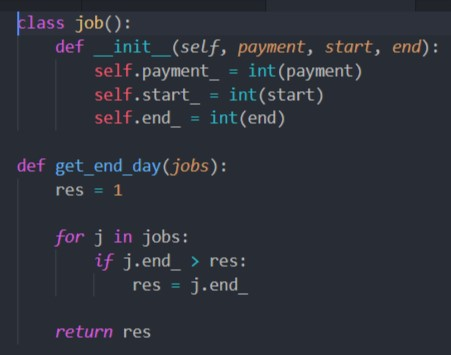
\includegraphics[trim=0cm 0cm 0cm 0cm, clip=true,scale=0.8]{figures/py_eg.jpg}
    \caption{Typical Python code snippet\label{Fig:pyeg}}\vspace{-4mm}
    \end{figure}

\paragraph{}
The Figure~\ref{Fig:pyeg} shows a typical python code example and Figure~\ref{Fig:wfgstruct} shows a WFG snippet. These two languages were built for two entirely different purposes but the highly adaptable nature of python makes a valid point whether if it can replace the functionality of WFG. But both languages have their pros and cons.

\subsubsection*{Python}
\paragraph{}
Python is a general purpose scripting language which focuses on user friendliness. It supports object oriented programming and is also backed up by a huge number of highly optimized libraries for various purposes. But when compared with languages such as C++ and Java, Python is heavy on the memory and slow for large volume computing. It is also not optimized for the particular purpose of programming the Wave DPU.

\subsubsection*{WFG}
\paragraph{}
WFG was created with one purpose and one purpose only in mind, Programming the Wave DPU. Thus it has primary operators that can precisely match the deep capabilities of the DPU hardware. It can be very efficient too when properly programmed. The downside to this language is that it is very strongly typed and is a user friendliness nightmare. Repetitive operators need to be manually entered by the user and the language has no capability of any kind of looping of the language itself.

\subsubsection{Python to WFG translator(Py2WFG)}
\paragraph{}
A solution was created by putting the best of both worlds together. The idea is to create a python 'sleeve' to cover up the WFG interface and present the user with a way to interact with python and get WFG level results. The user will now write up the script and when he runs it, it will output a fully optimized WFG script. 

\begin{figure}[H]
    \centering
    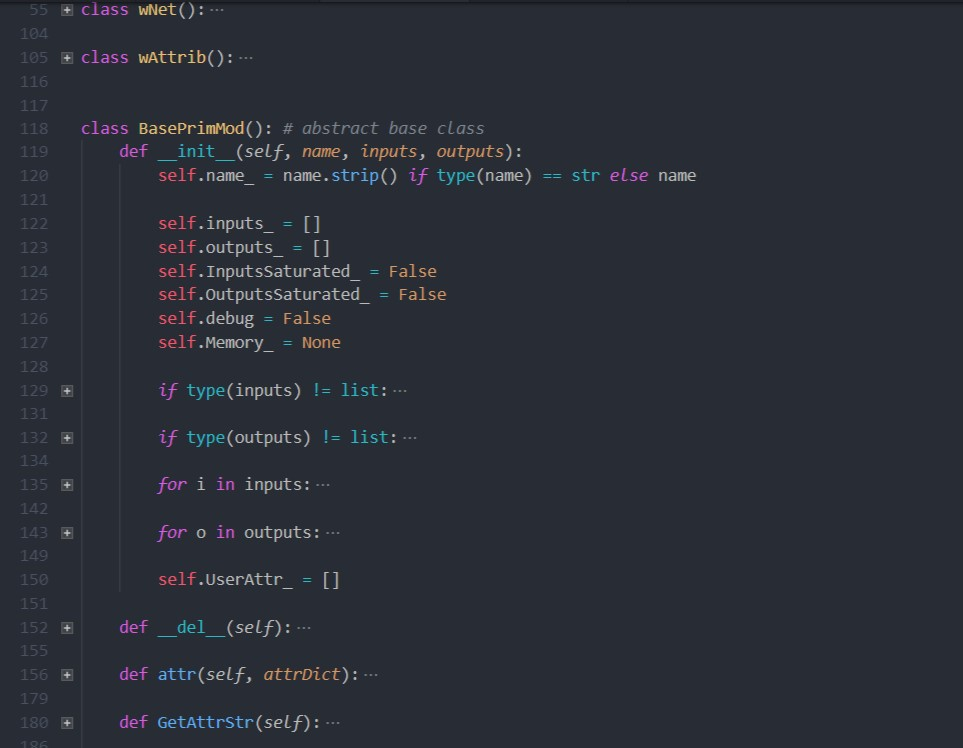
\includegraphics[trim=0cm 0cm 0cm 0cm, clip=true,scale=0.6]{figures/py2wfg_src.jpg}
    \caption{Part of the Py2WFG source code\label{Fig:py2src}}\vspace{-4mm}
    \end{figure}

\subsubsection*{Code Translation}
\paragraph{}
The basic idea for this library is derived from Tensorflow~\cite{tflow}, which is a python library that allows easy neural net design using a python library. The user will still need a sufficient knowledge on WFG syntax to use the library. But it will eliminate the hassles of writing a slightly-above-assembly language scripts by hand. The script that user needs to write is similar to the one showed in Figure~\ref{Fig:py2eg}. The library needs to be imported in to the script, Then Modules can be created from the wMod class in the library. These module 'husks' are then filled with dataflow operations as needed. When complete, issuing the makeWFG command will write a full WFG script that can be later integrated into the existing wave design flow.

\begin{figure}[H]
    \centering
    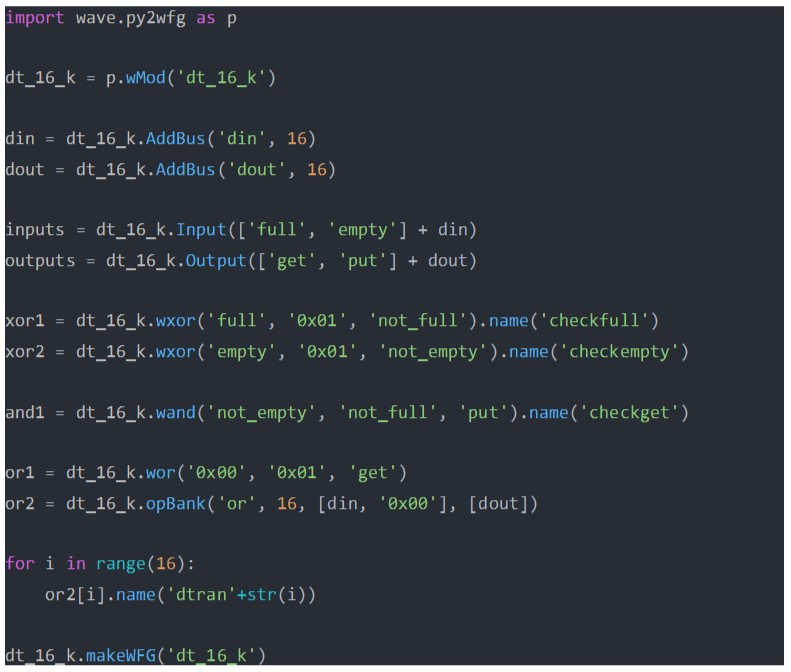
\includegraphics[trim=0cm 0cm 0cm 0cm, clip=true,scale=0.7]{figures/py2wfg_eg.jpg}
    \caption{Example Py2WFG script\label{Fig:py2eg}}\vspace{-4mm}
    \end{figure}

\paragraph{}
Running the example script shown in Figure~\ref{Fig:py2eg} will output a WFG file that contains the operations represented in the script, which is shown in Figure~\ref{Fig:wfgout}

\begin{figure}[H]
    \centering
    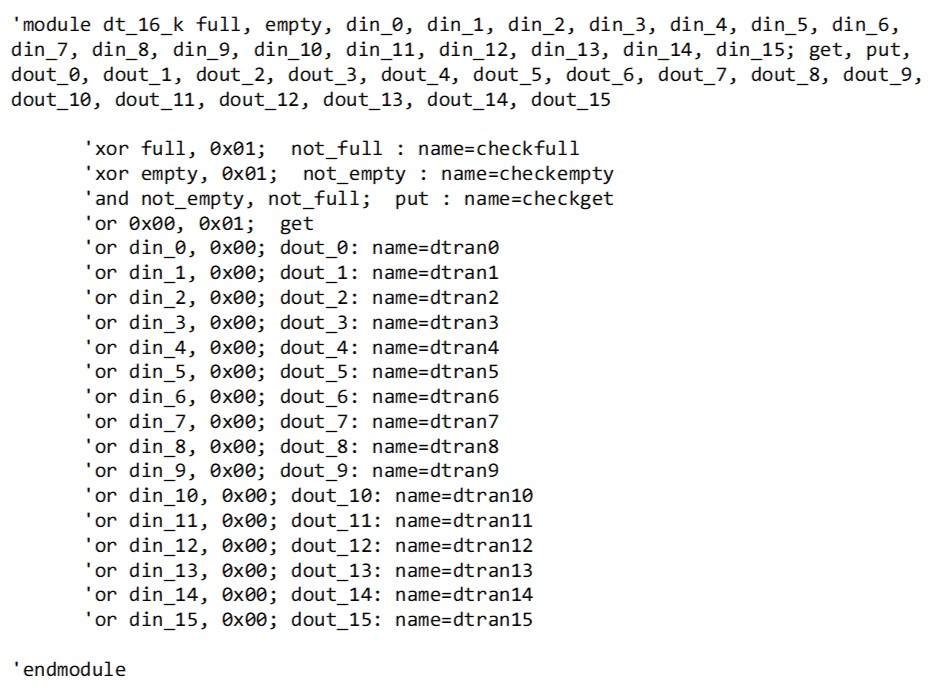
\includegraphics[trim=0cm 0cm 0cm 0cm, clip=true,scale=0.5]{figures/wfg_out.jpg}
    \caption{Output of the Py2WFG code from Figure~\ref{Fig:py2eg}\label{Fig:wfgout}}\vspace{-4mm}
    \end{figure}

\paragraph{}
This output WFG script unlike the handwritten scripts, is properly formatted and can be reconfigured easily through the python script again. This ease of use further improved with the introduction of the Simulator (section~\ref{sec:py2wfgsim}).

\subsubsection{Library Structure}
\subsubsection*{Data Types}
Main data types used in modeling a WFG module using Py2WFG are,
\begin{itemize}
    \item Primitive
    \item Pseudo
    \item Module
    \item Net
\end{itemize}

\subsubsection*{Primitive}
\paragraph{}
Primitives are basically WFG dataflow operations such as and, or, xfers, channel. These usually have inputs, outputs and attributes, depending on the specific primitive. These are the primary building blocks of a module.

\subsubsection*{Pseudo}
\paragraph{}
These are used for depicting memory operations such as ram and rom. They have connections different from dataflow operations but still have attributes just like dataflow.

\subsubsection*{Module}
\paragraph{}
Primitives and Memory get together to form modules. A module can correspond to a single WFG file or in more complex designs, several instances of one module can be created inside another module to form a hierarchical design.

\subsubsection*{Net}
\paragraph{}
These are somewhat similar to wires. They are used to interconnect modules and primitives. A collection of nets, grouped together for a common purpose is known as a bus.

\subsubsection{Python to WFG Simulator}
\label{sec:py2wfgsim}

\paragraph{}
The simulation of flow graph files are now done through WFGsim (section \ref{sec:wfgsim}). This platform is very complex and simulating a design on it takes a lot of overhead. To avoid this, an idea came up to add the ability to simulate Flow Graph designs on the Py2WFG library itself. This would allow the user to quickly write up a design on python and without exiting the python shell, they could quickly and efficiently simulate the design. 

\paragraph{}
Before calling up the simulator, if you need to test your designs against custom inputs, you need to define them in a special file called a input/output vector (iov) file.

\begin{figure}[H]
    \centering
    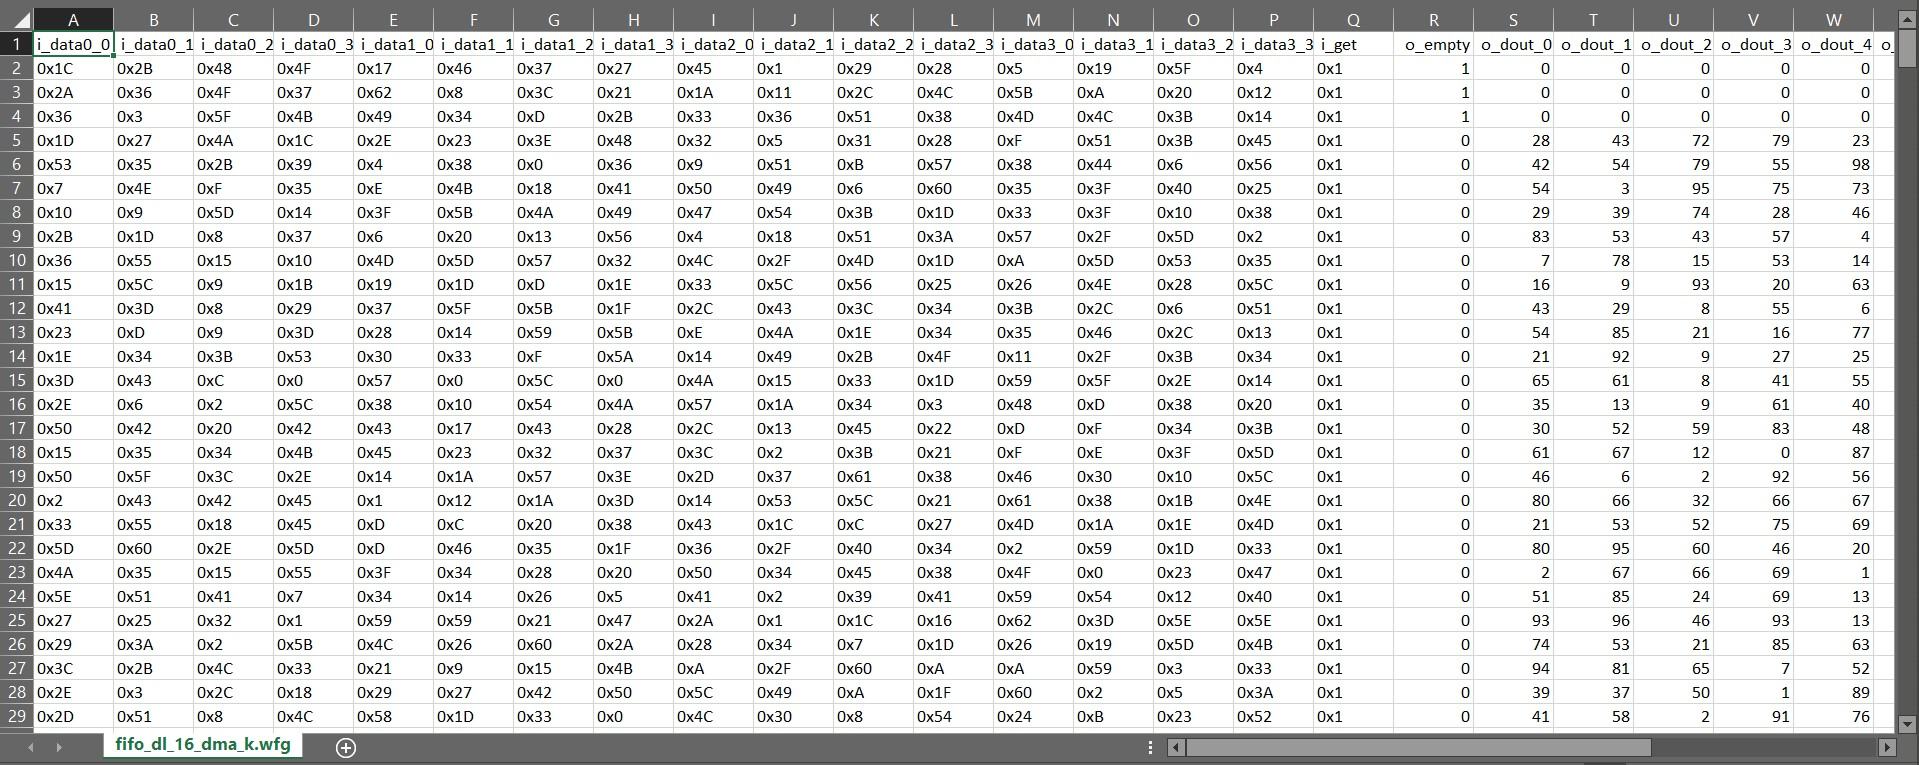
\includegraphics[trim=0cm 0cm 0cm 0cm, clip=true,scale=0.4]{figures/iov.jpg}
    \caption{A typical IOV file\label{Fig:iov}}\vspace{-4mm}
    \end{figure}

\paragraph{}
The values in Figure~\ref{Fig:iov} show the I/O values to and from the design in each tick the design was run for. The values that start as '0x' are input values, fed in hexadecimal format. Other values are the outputs which are in the decimal format. this is how WFGsim works, taking values in hexadecimal format and outputting results in decimal. 

\paragraph{}
Py2WFGsim can accept values in any base but it is also configured to mimic the behavior of WFGsim by default. It will look for this iov file upon startup, and if found, will simulate the design with those inputs and if unable to find this file, will generate a user configurable number of random input vectors (1000 by default) and run the simulation on them. User also has the option to define expected outputs for a given set of inputs and test it against the actual outputs. This makes Py2WFGsim a strong verification tool.

\begin{figure}[H]
    \centering
    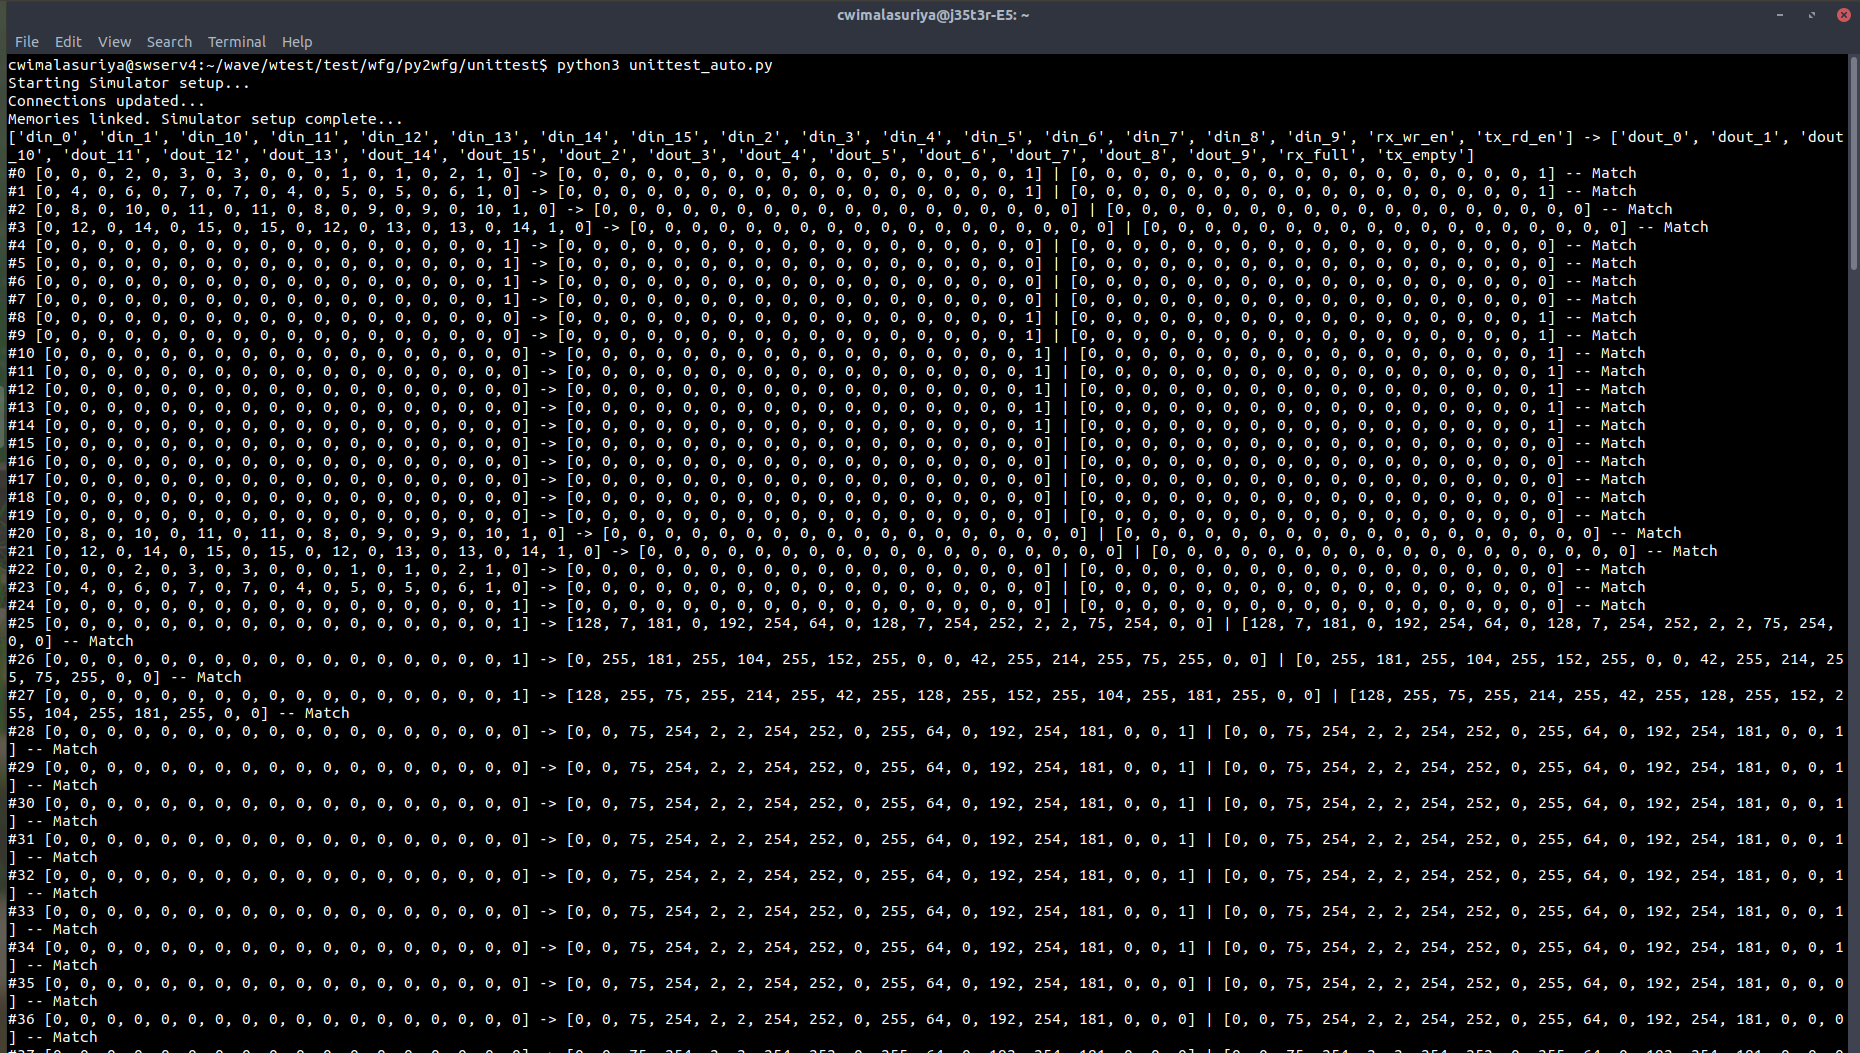
\includegraphics[trim=0cm 0cm 0cm 0cm, clip=true,scale=0.3]{figures/sim_result.png}
    \caption{Py2WFGsim user interface\label{Fig:simresult}}\vspace{-4mm}
    \end{figure}

\subsubsection{DMA engine}
\paragraph{}
The last part of the Project was implementing the DMA engine which was also the most controversial part since even now the engineers are having trouble with how this works. It is also known to slow down WFGsim and cause crashes and mismatches of all kind.

\begin{figure}[H]
    \centering
    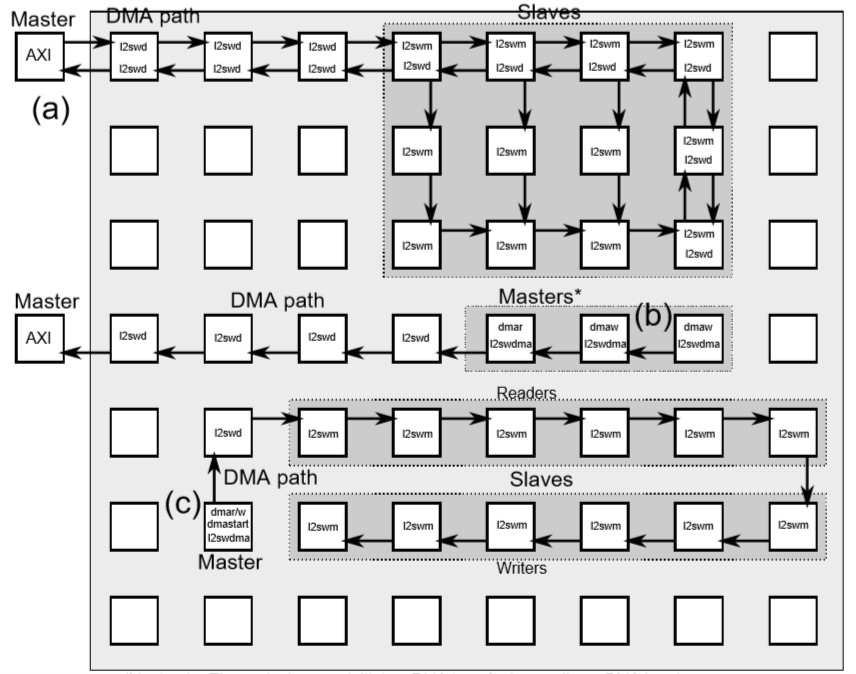
\includegraphics[trim=0cm 0cm 0cm 0cm, clip=true,scale=0.5]{figures/dma_path.jpg}
    \caption{Wave DPU DMA path\label{Fig:dmapath}}\vspace{-4mm}
    \end{figure}

\paragraph{}
DMA controller needs to be capable of communicating with an external host and managing the data transfers within the chip. These transfers are asynchronous and can occur at any time, making it highly challenging to implement it in a software based platform. Therefore, we decided that the DMA transactions and processing of data do not need to be executed in parallel for the time being. Another important decision is to altogether eliminate multi-thread programming, because it was identified as one of the major culprits of the poor performance in the original WFGsim. We opted for a linear implementation where only one operation executed at one time.

\paragraph{}
The final implementation consisted of standalone hosts that user can create and link to the channels of the design. Then the host would have R/W queues for each channel which it would properly execute as the time in the simulator passes by. This allows the user to freely schedule the host behavior without considering complex timing constraints. This design was successfully integrated to the simulator and it got accepted by the SDK team as a capable tool.

\subsubsection{Unit Testing}
\label{sec:unittest}
\paragraph{}
After building the simulator, a need arose to build a verification framework to test the translator and simulator libraries against new changes. To meet this requirement, a number of most used basic operators and a pair of complex WFG designs were put together to form a unit testing framework, which can be instantly called and the designs would be automatically verified and a report will be displayed. An example report is given in Figure \ref{Fig:utest}

\begin{figure}[H]
    \centering
    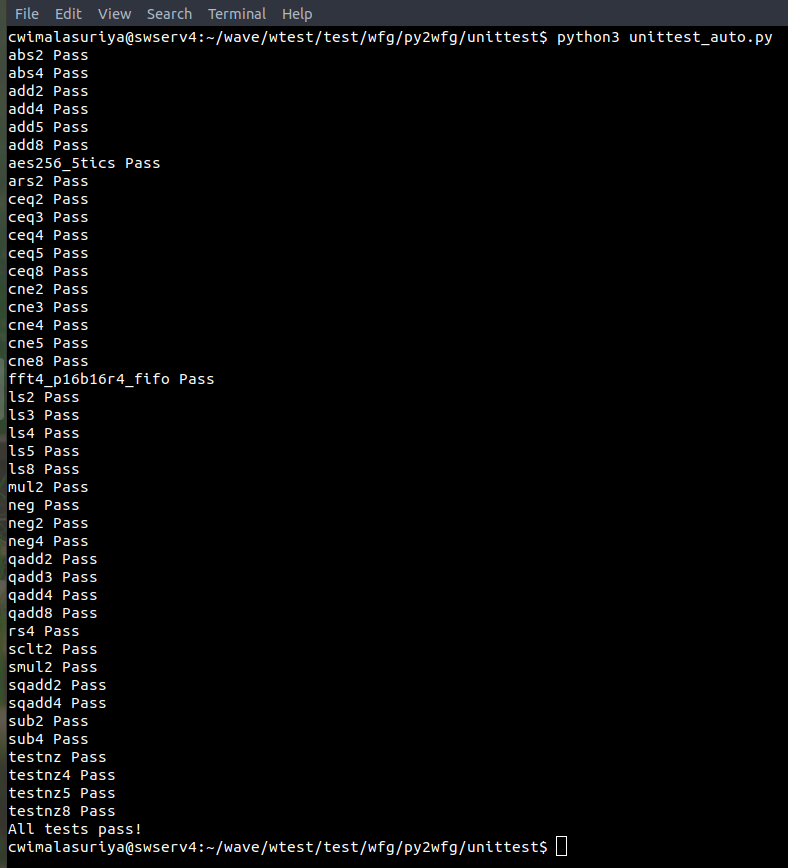
\includegraphics[trim=0cm 0cm 0cm 0cm, clip=true,scale=0.5]{figures/utest.png}
    \caption{Unit test framework report\label{Fig:utest}}\vspace{-4mm}
    \end{figure}

\subsubsection{International Testing}
\paragraph{}
To test out the translator/Simulator functionality, I was facilitated with a testing team consisting of people working from different countries including USA and China.

\begin{figure}[H]
    \centering
    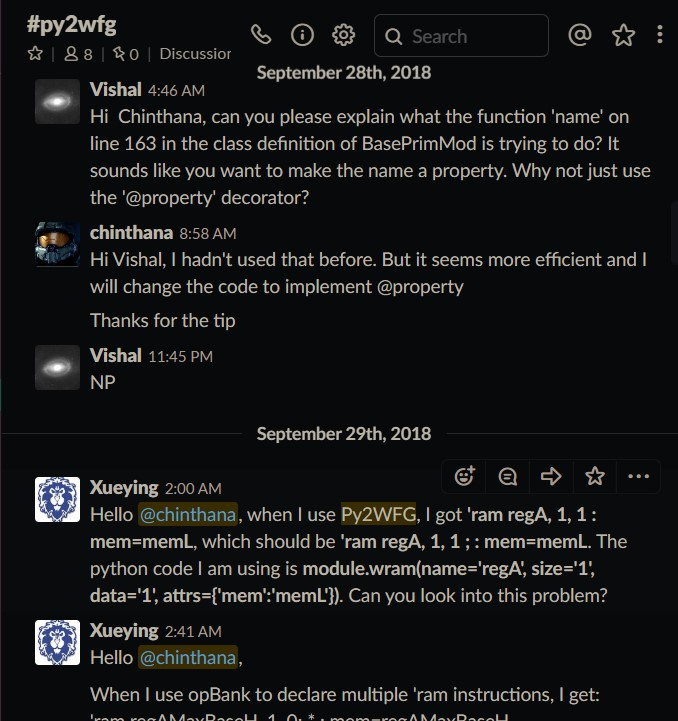
\includegraphics[trim=0cm 0cm 0cm 0cm, clip=true,scale=0.5]{figures/global_team.jpg}
    \caption{Communications with the overseas testing team\label{Fig:globalteam}}\vspace{-4mm}
    \end{figure}

\paragraph{}
This testing team was always helpful and efficiently reported whatever issues that the original designs had and came up with suggestions on best ways to solve the problems. They were a novel experience to me since I had never worked with a team scattered around the globe. It was rather efficient due to the software delivery system Wave has in place, allowing me to quickly deliver a fully tested builds of software to people in USA or China.